\section{\textbf{Supervised\\ Improve the Basic Classifier}}

%%%%%%%%%%%%%%%%%%%%%%%%%%%%%%%%%%%%%%%%%%%%%%%%%%%%%%%%%%%%%%%%%%%%%%%%%%%%%%%%
\begin{figure}[!ht]
    \centering
    \begin{subfigure}[b]{0.225\textwidth}
        \centering
        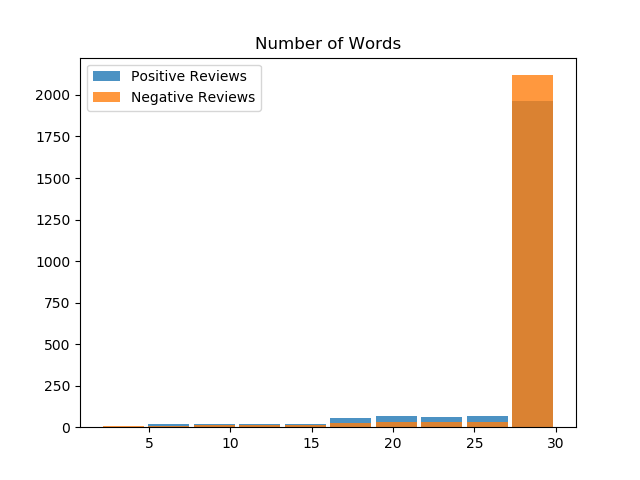
\includegraphics[width=\textwidth]{files/figs/ReviewWord.png}
        \caption[]%
        {{\small Number of Words}}    
        \label{fig:numberofwords}
    \end{subfigure}
    \hfill
    \begin{subfigure}[b]{0.225\textwidth}  
        \centering 
        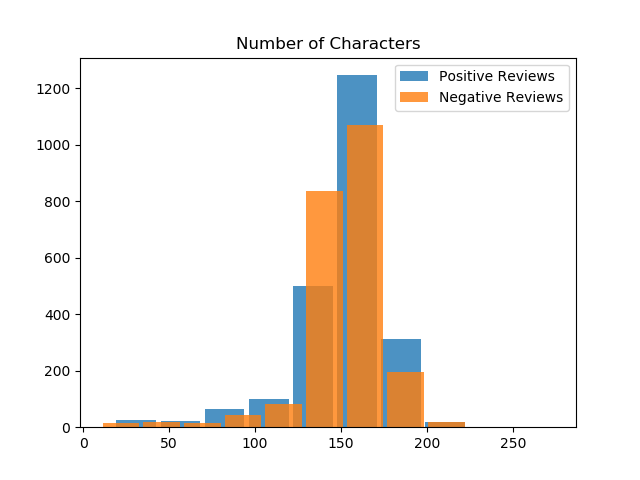
\includegraphics[width=\textwidth]{files/figs/ReviewCharacter.png}
        \caption[]%
        {{\small Number of Characters}}    
        \label{fig:numberofcharacters}
    \end{subfigure}
    \vskip\baselineskip
    \begin{subfigure}[b]{0.225\textwidth}   
        \centering 
        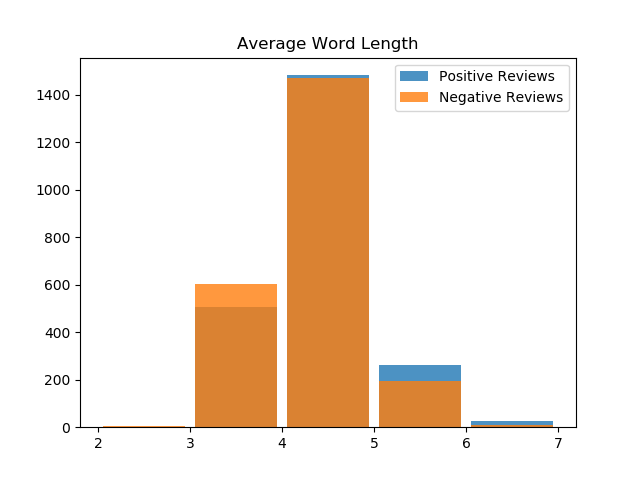
\includegraphics[width=\textwidth]{files/figs/AverageWordLength.png}
        \caption[]%
        {{\small Average Word Length}}    
        \label{fig:averagewordlength}
    \end{subfigure}
    \quad
    \begin{subfigure}[b]{0.225\textwidth}   
        \centering 
        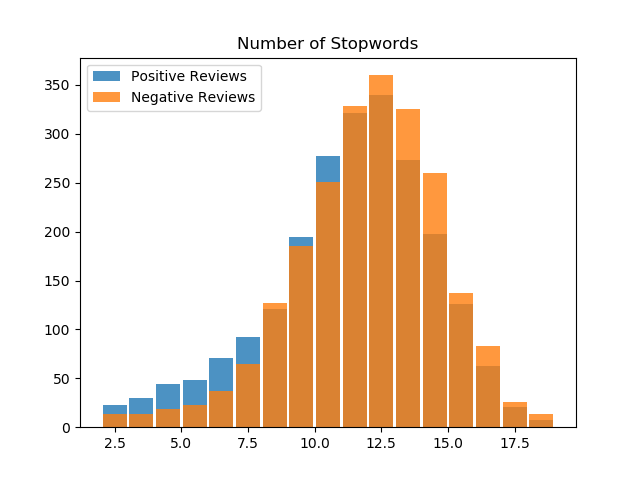
\includegraphics[width=\textwidth]{files/figs/NumberOfStopWords.png}
        \caption[]%
        {{\small Number of Stopwords}}    
        \label{fig:numberofstopwords}
    \end{subfigure}
    \caption[]
    {\small Some basic statistical information about dataset distribution.} 
    \label{fig:distribution}
\end{figure}

\subsection{\textbf{Basis Analysis of Dataset}}

After reading the data set, to perform different tasks on it, we should first perform some basic analysis on the dataset distribution. There are lots of features we can consider, like words, characters, stopwords, special characters, numerics, uppercase words and so on. Here due to limited time and resources, we only select a few indicators to illustrate the problem.

\subsubsection{Number of Words}

One of the most basic functions we can extract from text data is the number of words in each sentence. The intuition behind this is that generally speaking, the negative sentiments should contain a lesser amount of words than the positive ones. 

From figure~\ref{fig:numberofwords}, we can clearly see that due to the reason that sentences are cut off when the word length is longer than 30, there aren't many differences between the distribution of positive reviews and negative reviews.

\subsubsection{Average Word Length}

We also present another feature that will calculate the average word length of each sentence. This can also potentially help us in improving our model. The results are shown in figure~\ref{fig:averagewordlength}.

\subsubsection{Number of Characters}

Generally speaking, when solving a Natural language processing problem, the first thing we should do is preprocessing. The preprocessing can include various operations like spelling correction, tokenization and remove stopwords. Before doing preprocessing, calculating the number of stopwords may give us some extra information that we might have been losing before. The results are shown in figure~\ref{fig:numberofstopwords}.


\subsection{\textbf{Basic Pre-processing}}

Before diving into text and feature extraction, we first clean the training data in order to obtain better features. I tried the following preprocessing steps: transform sentences into lower case, removing punctuations, removing stopwords, common words, and rare words. I also tried different tokenizations. % However, each time I do preprocess, the performances become worse. 

\subsection{\textbf{Feature Engineering}}

Now we have done all the basic preprocessing steps to clean our data. Now, we move on to extract features.

\subsubsection{Term frequency}

Term frequency (TF) is simply the ratio of the count of a word represented in a sentence to the length of the sentence.

\subsubsection{Inverse Document frequency}

The intuition behind inverse document frequency (IDF) is that a word is not of much use if it's occurred in all the sentences. The IDF of each word is the log of the ratio of the total number of sentences to the number of sentences in which that word is present.

\subsubsection{Term frequency - Inverse Document frequency}

TF-IDF is the multiplication of the TF and IDF which we calculated above. TF-IDF can penalize commonly occurring words. We implement this feature using \textit{TfidfVectorizer} from \textit{sklearn.feature\_extraction.text}.

\subsubsection{Bags of Words}

Bag of Words (BoW) refers to the presentation of text which describes the presence of words within the text data. The intuition behind this is that two similar text fields will contain similar kind of words, and will have a similar bag of words. We implement this feature using \textit{CountVectorizer} from \textit{sklearn.feature\_extraction.text}.


\subsection{\textbf{Performances}}

\begin{table}[ht]  %table 里面也可以嵌套tabular,只有tabular是不能加标题的
\centering  %表格居中
\caption{Supervised Performances}
\begin{tabular}{lccc}
\hline
&    \textbf{BoW} & \textbf{BoW+TFIDF} & \textbf{BoW+TFIDF+Tuned \textit{LR}}\\
\hline
 \textbf{Train}   & 0.9997 &  0.9860 &  \textbf{1.0}   \\
 \textbf{Dev} &  0.7795 &  0.7773  &  \textbf{0.7948}   \\
\hline
\end{tabular}
\label{tab:supervised}
\end{table}

We created a model pipeline and performed an exhaustive hyperparameter search using \textit{GridSearchCV} from \textit{sklearn.model\_selection}. Some of the performances can be found in figure~\ref{fig:hyper}.

\begin{figure}[!ht]
    \centering
    \begin{subfigure}[]{0.225\textwidth}
        \centering
        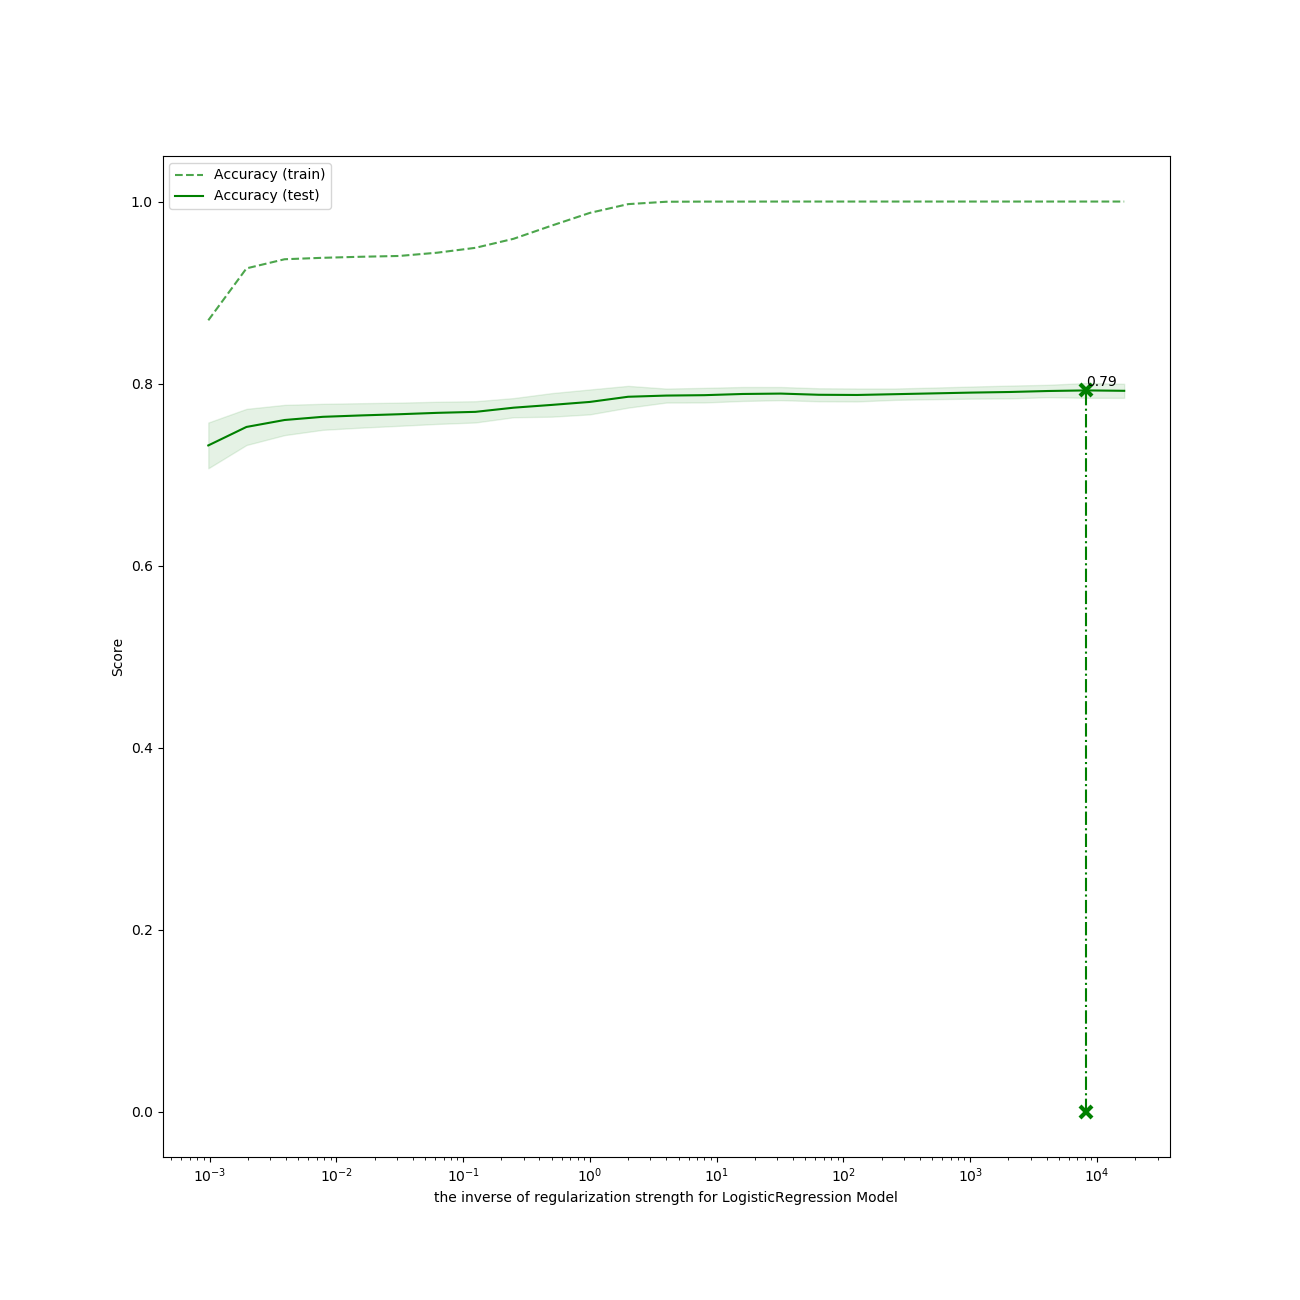
\includegraphics[width=\textwidth]{files/figs/finetuneC.png}
        \caption[]%
        {{\small Fine-tuned on regularization strength}}    
        \label{fig:numberofwords}
    \end{subfigure}
    % \hfill
    \begin{subfigure}[]{0.225\textwidth}  
        \centering 
        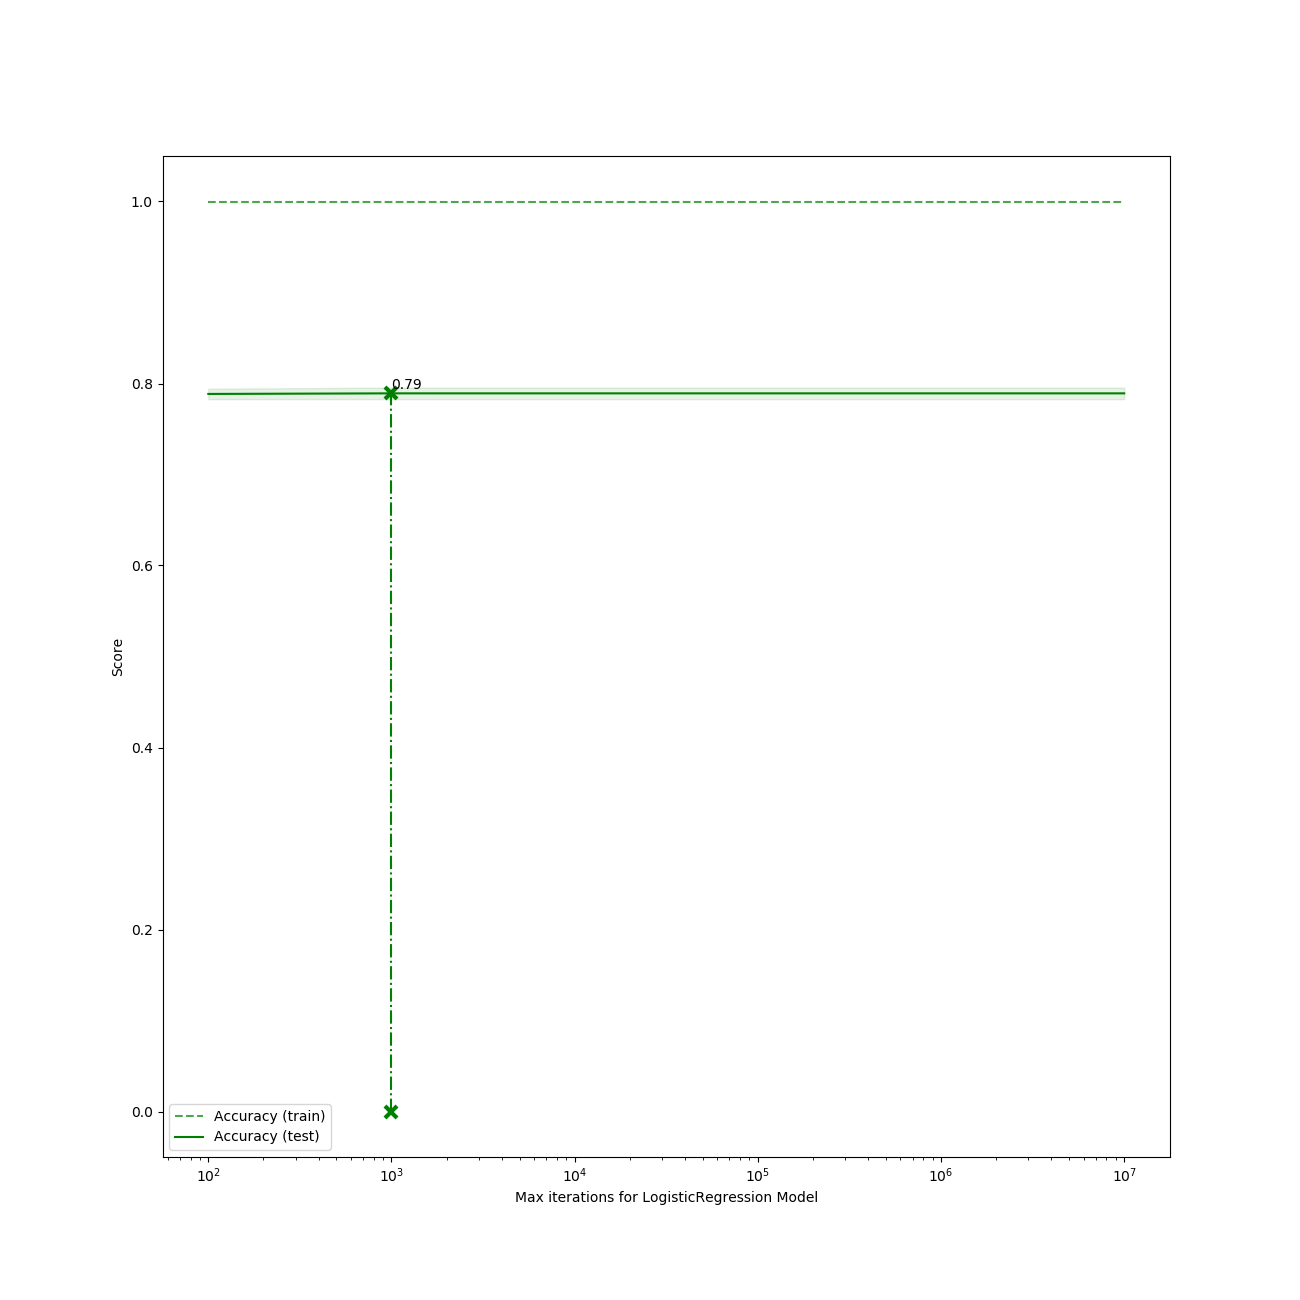
\includegraphics[width=\textwidth]{files/figs/finetuneIterations.png}
        \caption[]%
        {{\small Fine-tuned on max iterations}}
        \label{fig:numberofcharacters}
    \end{subfigure}
    \caption[]
    {\small Model performances on different hyperparameter settings.} 
    \label{fig:hyper}
\end{figure}

\begin{table}[ht]  %table 里面也可以嵌套tabular,只有tabular是不能加标题的
\centering  %表格居中
\caption{HyperParameters}
\begin{tabular}{lc}
\hline
&    \textbf{Parameters}\\
\hline
 \textbf{\textit{CountVectorizer}}   & \textit{max/min\_df, ngram\_range, stop\_words} \\
 \textbf{\textit{TfidfVectorizer}} &  \textit{use\_idf, smooth\_idf, sublinear\_tf} \\
 \textbf{\textit{LogisticRegression}} &  \textit{C, solver, max\_iter, class\_weight} \\
\hline
\end{tabular}
\label{tab:supervised}
\end{table}

The best performances were acheived under
\begin{itemize}
\item \textit{ngram\_range=(1,3)}
\item \textit{use\_idf=True}, \textit{smooth\_idf=False}
\item \textit{C=512}, \textit{solver='saga'}, \textit{max\_iter=1000}
\item DO NOT use any preprocess
\item DO NOT remove stopwords
\end{itemize}

From our experiments, we know that features from count-based vectorization methods like BoW and TF-IDF have some disadvantages:

\begin{enumerate}
\item They describe sentences by word occurrences while completely ignoring the relative position information of the words in the sentence (despite using N-grams, which is only a quick fix). 
\item TF-IDF word vectors are usually very high dimensional.
\item They are not able to capture semantics.
\end{enumerate}


